%%%%%%%%%%%%%%%%%%%%%%%%%%%%%%%%%%%%%%%%%%%%%%%%%%%%%%%%%%%%%%%%%%%%%%%%%%%%%%%%
%2345678901234567890123456789012345678901234567890123456789012345678901234567890
%        1         2         3         4         5         6         7         8

\documentclass[ 5p, 12pt, times, twocolumn, sort&compress ]{elsarticle}
\usepackage{ecrc}
%%%%\documentclass[letterpaper, 10 pt, conference]{ieeeconf}  % Comment this line out if you need a4paper

%\documentclass[a4paper, 10pt, conference]{ieeeconf}      % Use this line for a4 paper

%%%%\IEEEoverridecommandlockouts                              % This command is only needed if 
                                                          % you want to use the \thanks command

%%%%\overrideIEEEmargins                                      % Needed to meet printer requirements.

% See the \addtolength command later in the file to balance the column lengths
% on the last page of the document

% The following packages can be found on http:\\www.ctan.org
%%\usepackage{graphics} % for pdf, bitmapped graphics files
\usepackage{epsfig} % for postscript graphics files
\usepackage{mathptmx} % assumes new font selection scheme installed
\usepackage{times} % assumes new font selection scheme installed
\usepackage{amsmath} % assumes amsmath package installed
\usepackage{amssymb}  % assumes amsmath package installed
\usepackage{color}

\usepackage{url}

\usepackage{todonotes}

%% TODO: Check which packages unnecessary
\usepackage{pifont}
\usepackage{natbib}
\usepackage{geometry}
\usepackage{fleqn}
\usepackage{graphicx}
\usepackage{txfonts}
\usepackage{hyperref}
\usepackage{lineno}
\usepackage[figuresright]{rotating}

\newcommand\note[1]{\todo[inline, color=red!40]{#1}}
\newcommand\mNote[1]{\todo[inline, author=Michael, color=cyan]{#1}}
\newcommand\maNote[1]{\todo[inline, author=Maor, color=green]{#1}}
\newcommand\rNote[1]{\todo[inline, author=Ronen, color=yellow]{#1}}

\definecolor{frameColor}{RGB}{204,204,204}

\usepackage{xcolor}
\usepackage{float}

\newcommand{\frameImage}[4]{
\begin{figure}[H] 
  \centerline{
    \fcolorbox{frameColor}{white}{
        \includegraphics[height=#2, width=#3]{#1} } }
    \caption{#4}
    \label{fig:#1}
\end{figure}
}


\definecolor{ColorNodeName}{RGB}{140, 56, 99}
\definecolor{ColorNodeInvariant}{RGB}{167, 66, 168}
\definecolor{ColorEdgeGuard}{RGB}{66, 168, 72  }
\definecolor{ColorEdgeProbability}{RGB}{168, 122, 66}
\definecolor{ColorEdgeUpdate}{RGB}{66, 66, 168}
\definecolor{ColorEdgeSynchronization}{RGB}{66, 160, 168}

\newcommand\colorsCellHeight {4}
\newcommand\colorsCellWidth  {10}

\newcommand\colorsTable  {
\begin{table}[H] 
\centering 
\begin{tabular}{|l|c|} \hline
\tiny Attribute               & \tiny Color\\ \hline
\tiny Node name               & \fcolorbox{ColorNodeName}{ColorNodeName}{\makebox(\colorsCellWidth,\colorsCellHeight){}} \\ \hline
\tiny Node invariant          & \fcolorbox{ColorNodeInvariant}{ColorNodeInvariant}{\makebox(\colorsCellWidth,\colorsCellHeight){}} \\ \hline
\tiny Edge guard              & \fcolorbox{ColorEdgeGuard}{ColorEdgeGuard}{\makebox(\colorsCellWidth,\colorsCellHeight){}} \\ \hline
\tiny Edge probability        & \fcolorbox{ColorEdgeProbability}{ColorEdgeProbability}{\makebox(\colorsCellWidth,\colorsCellHeight){}} \\ \hline
\tiny Edge update             & \fcolorbox{ColorEdgeUpdate}{ColorEdgeUpdate}{\makebox(\colorsCellWidth,\colorsCellHeight){}} \\ \hline
\tiny Edge synchronization    & \fcolorbox{ColorEdgeSynchronization}{ColorEdgeSynchronization}{\makebox(\colorsCellWidth,\colorsCellHeight){}} \\ \hline
\end{tabular} 
\end{table}
}

% TODO: 
\volume{105}
\firstpage{56}
\journalname{Robotics and Autonomous Systems}
\runauth{}
\jid{procs}
\jnltitlelogo{Procedia Computer Science}


\begin{document}

\begin{frontmatter}

\dochead{}
%%%\maketitle

\title{\LARGE \bf Performance Level Profiles: A Formal Language for Describing the Expected Performance of Functional Modules}


\author[braf]{Ronen I. Brafman}
\ead{brafman@cs.bgu.ac.il}

\author[kova]{Alexander Kovalchuk}
\ead{alex.cs.rnd@gmail.com }

\author[ashk]{Maor Ashkenazi}
\ead{maorash@cs.bgu.ac.il}

\author[bar]{Michael Bar-Sinai}
\ead{barsinam@cs.bgu.ac.il}

\address[braf,kova,ashk,bar]{Department of Computer Science, Ben-Gurion University, Beer-Sheva, Israel}
       % {\tt\small \{brafman,barsinam,maorash\}@cs.bgu.ac.il and alex.cs.rnd@gmail.com } }%

%%\thispagestyle{empty}
%%\pagestyle{empty}


%%%%%%%%%%%%%%%%%%%%%%%%%%%%%%%%%%%%%%%%%%%%%%%%%%%%%%%%%%%%%%%%%%%%%%%%%%%%%%%%
\begin{abstract}

Despite the existence of powerful formal languages for writing robot controllers, most existing functional modules are written using standard
programming languages. The existence of such a code base raises critical challenges: 1. How to enable automated analysis, monitoring, and reuse of existing code given that reasoning directly about code fragments is  impractical. 
2. How to convey to users the expected level of performance of an autonomous robot?
3. How to estimate the outcome of a complex script or controller for a task?
4. Perhaps most crucial: how to quickly identify abnormal behaviour of autonomous robots? This is a key impediment to the
deployment of such platforms in open environments.
In this paper we describe {\em performance-level profiles (PLPs)\/}, a formal, yet intuitive, 
language for specifying the expected properties of functional modules, designed with the above aims in mind. 
PLPs are motivated by action specification languages, such as PDDL 2.1,
but add novel elements important for robotic applications, such as update frequency, run-time statistics, progress measures, and trigger conditions, 
and take into account the different roles modules can play. We describe the language, a formal semantics for it using probabilistic time automata, and
explain how it is used to aid in online monitoring and verification of code. We describe software available in support of these goals and its
use in two projects: an autonomous compact track loader, and a service robot. 


\end{abstract}

\begin{keyword}
PLP
\end{keyword}


\end{frontmatter}

%%%%%%%%%%%%%%%%%%%%%%%%%%%%%%%%%%%%%%%%%%%%%%%%%%%%%%%%%%%%%%%%%%%%%%%%%%%%%%%%


\section{INTRODUCTION}

The robotics research community has made much progress designing software engineering tools that make it easier to develop
robotic modules and controllers (e.g.,~\cite{PRS,TCA,RPML} to name a few). Many of these tools (e.g., BIP~\cite{BIP,BIP2}) are based on formal concepts and formal languages that provide  guarantees about the properties of the resulting code, and constructs for composing
different modules. An ideal situation would be for practitioners to adopt such technology. Yet, in practice, functional modules are often simply coded
by programmers using conventional software practices and languages.
%, even if on top of infrastructure such as ROS. 
%This makes it difficult to reach an ideal plug-and-play state, where one can program a robot by assembling pre-existing modules. 
Unfortunately, as noted in~\cite{Abdellatif12}:  "Systems built by assembling together independently developed and delivered components often exhibit pathological behavior. Part of the problem is that developers of these systems do not have 
{\bf a precise way of expressing the behavior of components\/} ..."
%at their interfaces, where inconsistencies may occur." 

Addressing this issue is crucial to our ability to deploy autonomous robots in open environments. 
Lacking a precise definition of normal behavior, how will we identify abnormal one? Certainly, we would not want to wait until 
%the last moment where 
some evidently undesirable outcome occurs, nor is the public likely to tolerate such performance.
Moreover, even before deployment, users would want to understand what they are getting 
before spending large amounts of money on an autonomous robot, or using some open-source package.

Yet another pragmatic consideration is that the lack of {\em machine readable\/} behavior specification prevents the development and
use of tools that utilize such specifications to {\em automatically\/} support monitoring, validation, and planning.
%Unfortunately, functional modules without clear formal semantics are difficult to combinen novel ways, as would befit an autonomous robot, which is offered by more principled formal tools.
%Given this state of affairs, if robotic infrastructure is to reach a plug-and-play state, as in personal computing, we must be able to combine diverse robotic modules and components easily, and automatically. Yet, 
%Moreover, what we ultimately would like to do is to have such modules assembled on-the-fly to address new tasks faced by an autonomous robot.
%


We encountered these needs in a project involving a large industrial partner, a professional service provider, and academic partners, seeking to build an autonomous compact track loader (CTL) for discovery and evacuation of land-mines. 
%
For the industrial partner, replacing its own code base and methodology was not an option, and it complained about the difficulty of marketing products without the ability to  provide clear performance guarantees to the CTL's functional modules. With different modules supplied by different partners, documented using the widely used text-based SSS (systems/subsystem  specification), it was difficult to foresee how each module would behave.
Moreover, various performance problems encountered at run-time were identified at a late stage, although with appropriate monitoring earlier warnings could have been issued.




%such as ROS, for useful services. Given such code, we would like to monitor its execution, validate that scripts that combine this code in
%various ways have certain desirable properties. Doing this manually is difficult, time consuming, and is appropriate only offline. Doing it automatically,
%is very difficult, if not impossible, given mere code. To that end, it is desirable to have machine-readable description of



%Web service and network infrastructure providers often sign service-level agreements (SLAs) with their users. These agreements describe  {\em minimal\/} commitments regarding the functionality of these services that the user can rely upon, providing the latter with some confidence and guidelines regarding what it can expect from the service. SLAs are not precise specifications of the service, but provide a good-enough abstraction for most users. We would like to suggest that a similar concept is useful and appropriate in the context of robotics, and especially autonomous robots.


Although it is difficult to provide a precise specification of the behaviour of a module given an open-ended world,%
\footnote{By "module" (often called "component") we mean a piece of software or hardware that provides some
functionality, whether low level, like a sensor, or higher level, such as a navigation package.}
%Starting with a sensor that provides raw data, a software module that generates some higher-level data from it,aimple code that generates basic motion, or more complex code that provides complex motion that is informed by some sensor input, or some higher level function, such as clearing a path of obstacles.}
it appears possible to provide a "good-enough" partial description of the module's role, the conditions under which it is expected to succeed, its success probability, and its expected running time (when relevant).

Motivated by these considerations, we define a language for specifying {\em performance-level profiles} or {\em PLPs}~\cite{PLP14}. PLPs describe a number of key aspects of the performance of functional modules. They combine 
ideas from planning language (PDDL 2.1~\cite{PDDL2.1}, probabilistic PDDL~\cite{YouLit04}, RDDL~\cite{RDDL}), diverse goal notions, such as achievement and maintenance goals~\cite{PRS, aamas07maint}, and new notions such as progress measures and a {\em repeat\/} construct
aimed at making explicit the frequency by which input parameters are read and output parameters are published. Unlike action languages that limit
their expressiveness to meet the requirements imposed by state-of-the-art planning technology, PLPs seek to provide expressiveness that can be used for other tasks, such as performance monitoring. They can also be viewed as extending the expressivity of contracts within the Design by Contract approach~\cite{Eiffel} 
% -- quite often an important parameter in the design of robotic modules that can influence various error parameters.

% can form the basis of performance level commitments by module designers, forming what can be called  {\em performance-level agreement (PLA)\/}. That is, a PLA is an agreement/commitment/contract in the form of a PLP.
%, that 
%closely resonate with issues we encountered during a joint project with industrial (Israel Air Industries and Cogniteam) and academic partners.
%First, our industrial partners complained about the lack of ability to provide customers with some reasonable performance guarantees. Second, it was evident that in a collaborative project, with 
%different modules supplied by different partners, it will be difficult to validate various sequences of operations, or to generate them automatically, without a suitable, formal specification of the functional modules. Third, although formal methods for development of modules with guarantees and clean specifications are available (e.g.,BIP~\cite{BIP}),
%it was  unrealistic to expect these practitioners to change their software development practices and software development tools for this project. PLPs were introduced to address these issues.

PLPs have a number of potential roles. At  design stage, PLPs can replace or supplement informal text-based specifications such as SSS.
%SSS are often used by system
%engineers to describe requirements from a software module. 
%SSS have rigid structure, but field content is textual. 
They can also be used to quantify the commitments made by module designers to module users, whether customers or other developers. Perhaps most importantly, PLPs outline expected behavior, so they can be used to {\em automatically\/} identify abnormal behavior, alerting the user or the system. Thanks to their structured, machine readable syntax, they can be manipulated 
automatically for the purpose of online monitoring, validation, and planning.

The goal of this paper is to describe PLPs, their semantics, and how they can help automate the task of generating monitoring code as well as verify complex behaviors. After describing PLPs, we describe their formal semantics. This is done by providing a mapping from PLPs to \textit{probabilistic timed automata} (PTAs)~\cite{}, a well known model that is used in program verification. Beyond its theoretical value, this mapping allows us to exploit existing tools for program verification. Moving from the mapping of
a single component into PTAS, we show how we can map complex programs that combine component by using
conditions, randomness, and parallelism, into PTAs.
Given these PTAs, we can now verify their properties.
We describe the software we built in support of these techniques: software for specifying PLPs, for automatically generating monitoring code from PLPs,
for learning online parameters of PLPs, and for verifying properties of programs, given PLPs for their basic components. 


%Third, automated reasoning tools can operate over these formal commitments: they can monitor whether
%the commitments are met only, and they can serve for the purpose of validation, and ultimately, automated planning
%In particular, we are working on simple tools that will make it very easy to use them as input to a third-party monitoring tool available for ROS.
%These tools make it easy to specify, initially, PLPs with abstract conditions, and to eventually turn them into
%conditions grounded in code.


\section{PLPs}
The primary objective of a PLP is to clarify the role and expected/normal behavior of a module. As a simple example, imagine a module designed to grasp an object. The expected outcome is that the object is held by the arm. However, in most realistic settings, this effect is not guaranteed. There is some probability of failure, and failure can come with some side effects, such as the object falling, or being broken. And while the running time is most likely not deterministic,  we can try to describe properties of its distribution. We can also describe its rate of progress. For instance, the grasping module is usually not static until the object is
captured, and so we expect its position to change at some minimal rate.
Moreover, the probability of success and failure may depend on various properties, such as the shape and size of the object.
Furthermore, in certain settings it may be unrealistic to specify the success probability, as too many external factors could impact it. For example, if another arm is attempting to catch the object at the same time, it may difficult to predict which one will succeed.

PLPs are described in XML-based format. Each XML document must conform to an XML Schema Definition (XSD) that describes the PLP's formal syntax -- with
one XSD for every PLP type: {\em achieve, maintain, observe, detect}. XML and XSD were chosen for their simplicity and wide-spread use and support. Any tool for editing XML and verifying its structure based on an XSD file can be used as a PLP editor. The precise syntax of the four schema
is laborious, and can be found in https://github.com/PLPbgu/PLP-repo together with an example of a PLP of each type. Below we provide an informal description of the information contained in the respective XML/XSD documents.
%\mNote{ for URLs, I suggest we use dataverse.harvard.edu. They offer free storage, support citations and doi etc.}
%\rNote{Fine with me, although something off our web pages would be fine too.}

\subsection{Overview}
PLPs have two abstract components. The first circumscribes the conditions under which the profile is provided -- conditions that must hold for it to be valid. Such conditions include various properties of the world before and during execution
as well as available resources. The second specifies the effect of the action -- what success means, what are the possible failure modes, what is the probability of each, what is the distribution over running times, and what is its rate of progress. More generally, it can specify a statistical profile of various aspects of normal module behavior at run-time. 

There are four PLP types, corresponding to four module types. {\em Achieve} modules attempt to achieve a new state of the world
or generate a new object. For example, changing the orientation of the robot to some goal orientation. {\em Maintain} modules attempt to maintain some property. For example, maintaining some orientation; or, ensuring that the robot remains within some confined area. 
%We allow for maintain modules that maintain a property that is not necessarily true initially.
%For example, "maintain speed of 10km/hr".  Thus, essentially, these modules need to make the condition true and maintain it.
%In principle, one could separate this into two phases: achieve, then maintain; but this separation is not natural in many cases, especially when the module is essentially a closed-loop controller that continuously attempts to reduce the difference between the current condition and the target condition. 
{\em Observe}  modules  attempt to recognize some property of the current state of the world. For example, the robot's location, or whether there is a cup on the table.
%\mNote{Not sure the cup is the best example - to me it sounds like detection of a cup}
%\rNote{Any boolean thing you can observe, you can detect too. The difference is in the time span. Detect a cup is essentially repeat observe(cup) with termination condition of being observed. If you ask me "is there a cup on the table" I use observe. If you tell me "let me know when there is a cup in the sink" then I use detect. But if you find the example confusing, we can change.}
Finally,  {\em Detect\/} modules monitor the state of the world until some condition holds.

Many robotic modules operate by repeatedly updating or modifying some data-structure or signal based on information that is
constantly being updated.
To model such constructs we introduce a {\em repeat\/} option for the {\em achieve\/} and {\em observe\/} modules. 
For example, 
%a mapping module constantly updates a map of the environment as it obtains information from relevant sensors,
%thus, it repeatedly observes. Similarly, 
a path-planning module may update the path as it obtains updated maps. It can be viewed as performing an {\em achieve\/} task repeatedly.%
%\footnote{With the introduction of {\em repeat} wrapper, one can argue that 
%{\em maintain} and {\em detect\/} become redundant, as {\em maintain\/} can be implemented as repeat-achieve, while {\em detect} can be implemented as repeat-observe. Nevertheless, we feel that this redundancy is worth the added modeling
%convenience.}


\subsection{Variables and Resources}
The formal definition of PLPs rests on the specification of properties of states of the world. 
These are defined by specifying properties of various state variables.
% It is desirable to have a coherent specification of such variables, so that the relationship between modules is clear. 
%The meaning of these variables -- their relationship to the real world, i.e., the correspondence between the model and the real world must be clear for the specification to be meaningful. Some state variables can refer to local system parameters, of course. 
%
In addition, each module may need access to certain resources. These resources could be energy or memory, some actuator, or some region of space. These must be specified, much like state variables, and coherent and consistent use of these names is required. In fact, resources can be viewed as a special class of state variables, whose state indicates the status of the resource (e.g., available, $> 100$ gallons, etc.). 
However, because they carry special significance to programmers and operators, we distinguish them from other variables. 

%Software support for consistent use and maintenance of the list of variables and resources is advisable and is part of the set of tools supporting PLPs that we are constructing.

\subsection{Common Elements}
All modules specify the following elements:

\noindent {\bf Parameters:} values supplied to the module as input or provided by the module as its output. Some input
parameters can also be output parameters (i.e., after undergoing some processing). One special class of parameters are {\em error\/} parameters. That is, parameters that specify the accuracy of other parameters. For example, if localization is performed using a Kalman filter, an error estimate can be obtained from its covariance matrix.

\noindent {\bf Set of variables:} Local variables and their range.

\noindent {\bf Application Context:} Conditions specifying the contexts in which the PLP is valid. It contains
the following elements:
\begin{itemize}
\item {\bf Required resources:} List of resources required. If the resource is quantifiable, a required quantity is mentioned.
If the resource is needed for operation and then freed (e.g., memory, some tool, some actuator), the requirement status must
be mentioned. Possible values are "exclusive" or some frequency of use.
\item {\bf (Optional) Maximal rate of change:} Maximal change in resource level per time unit.
\item {\bf Preconditions:} conditions on the world at the start of execution time under which the PLP is defined. These conditions can refer only to parameters.
\item {\bf Concurrency conditions:} conditions on the world at execution time under which the PLP is defined. 
%These can be on parameters as well as local variables.
They can also refer to the rate of change of parameters. For example, stating that successful
navigation requires respecting some maximal speed limit.
\item  {\bf Concurrent modules:} conditions on modules that must or must-not be executed concurrently.
%These fields specify the conditions under which the PLP is defined. That is, a PLA based on
%this PLP makes no guarantees if these 
%conditions are violated.
\item  {\bf (optional) Parameter frequency:} The frequency by which each parameter must be read or written. 
%For example, localization information may be required throughout the execution of  various navigation tasks. 
The frequency by which a parameter is updated together with its accuracy (which is available if an error parameter exists)
can affect the accuracy of output. For example, a navigation module that aims to reach a specified position may need to obtain position information with certain rate and certain accuracy to ensure success.
\end{itemize}
%Semantically, {\em required resources\/} ?
%as well as {\em maximal rate of change\/} 
%is a special types of concurrency conditions. It does not describe resource consumption, though, which one should 
%specify in the  {\em side-effects\/} field.

\noindent {\bf Side-effects:} Each module has an intended effect, or role. However, it may also have side-effects that are a result of executing this module, but are not a measure of its success or failure. For example, if the module consumes some resource, a natural side effect is that the level of this resource 
is reduced. Side effects are described by a conditional assignment to a parameter, which could depend on a local variable (such as running time, or distance traveled). Intuitively, side-effects are changes caused by the module that could potentially impact other modules.

\noindent {\bf Expected Progress Rate:}  Some modules perform continuous work to achieve or maintain their goals.
For example, when navigating, the position will change at some rate as long as the robot is not at its destination.
Or, when grasping an object, the hand will move closer to the object. In this field, one specifies
the minimal rate of change per time unit, as well
as the time unit itself (e.g., $\Delta(x)\geq 1$ meter every 1 minute).
Making these expectations explicit makes it easier to recognize problematic behaviour while the module executes.


\subsection{PLP Types}
There are four types of PLPs: {\em achieve, maintain, observe, detect}.
We briefly describe each type. 
%See the link provided earlier for more information.
See https://github.com/PLPbgu/PLP-repo for more information.


{\em Achieve\/} modules attempt to reach a state of the world in which some desirable property holds. For example,
fuel tank is full, robot is standing, plane has landed, etc. Achieve also covers cases where the goal
is to generate some virtual object, such as a map or a path.
Beyond the common elements, their PLP contains
the following:  the achievement goal -- a boolean condition defined over suitable parameters, 
failure modes -- which are various ways the module could fail to achieve the goal, the probabilities associated with
success and each failure mode, and the running time distribution given success and given failure. 
%\noindent {\bf  (optional) Failure modes:} Possible ways in which the module could fail to achieve the goal. That is, these are conditions that are inconsistent with the achievement goal that could be the outcome of the action.

%\noindent {\bf  Probability of success.} It may be conditional on properties of the world, and expressed via parameters.

%\noindent {\bf  Failure probability:} For each failure mode, its probability, possibly conditional on some parameter values.

%\noindent {\bf  Running time distribution given success.} Possibly conditional on various parameters, e.g.,
%Rayleigh(f(path-length)]

%\noindent {\bf  Running time distribution given failure.} Possibly conditional on various parameters,  e.g.,
%Rayleigh(g(path-length)]

%\noindent {\bf Example}: achieve "holding(cup)"
%\begin{itemize}
%\item Set of parameters: arm-empty, wet(cup), clear-path(cup)
%\item Achievement goal: holding(cup)
%\item Requires resources: robot-arm (exclusive)
%\item Preconditions: arm-empty, clear-path(cup), cup-ok
%\item Concurrency conditions: none 
%\item Concurrent modules: none
%\item Side effects: $\neg$arm-empty
%\item Failure modes: (1) $\neg$holding(cup) (2) $\neg$holding(cup) and broken(cup)
%\item Probability of success: 0.9 if $\neg$wet(cup), 0.3 if wet(cup)
%\item Failure probability: (1) 0.08 if $\neg$wet(cup), 0.4 if wet(cup) (2) 0.02 if $\neg$wet(cup), 0.3 if wet(cup)
%\item Running time  given success: Normal(60,20).
%\item Running time  given failure: Normal(80,40).
%\end{itemize}
%

%\subsection{Maintain Modules}
{\em Maintain\/} modules attempt to maintain the value of a variable or the truth value of a boolean condition,
e.g., maintain heading, maintain speed, maintain perimeter clean. The condition need not be true initially, 
and so the module may need to initially attain the condition, as in a closed-loop controller that always attempts to
decrease some distance to the desired goal condition. For this reason we do force users to split such
cases into {\em achieve} and then {\em maintain} -- our goal is to describe code, not to force a certain architecture.  

In addition to common elements, the PLP of {\em maintain} modules contains: the condition to be maintained,
whether it is initially true, termination conditions, one for successful termination and one for failure,
failure modes, the probability of successful termination and different failure modes, and the runtime distribution given success and failure.
A success termination condition is not necessary, and the run-time distribution will often be memoryless (i.e., exponential).
%
%\noindent {\bf Maintained condition} Defined over parameters. 
%
%\noindent {\bf Initially true?} A boolean value that indicates if the module expects the condition to be true initially.%
%%\footnote{Formally, this is just another precondition. But because of its central role, it is designated as a special field.}
%
%\noindent {\bf Success Termination condition:} Condition under which module stops operating (could be time). This is a condition that does not violate the maintenance goal.
%
%\noindent {\bf Failure Termination conditions:} Conditions under which module stops operating (could be time). These are conditions that indicates some type of failure. There may be multiple such conditions.
%
%\noindent {\bf (optional) failure modes:} Possible ways in which the module could fail to maintain the condition.
%
%\noindent {\bf Probability of success.} Possibly conditional on properties of the world.
%
%\noindent {\bf Failure probability.} For each mode, probability may be conditional on properties of the world.
%
%\noindent {\bf Running time distribution given success.} Can be conditional on other parameters.
%
%\noindent {\bf (optional) Running time distribution given failure.} Can be conditional on other parameters.
%

Sometimes, one needs to maintain some condition in order to achieve a goal. For example, one may reach a 
target position by maintaining a pre-computed path to the goal, either by iteratively reaching way-points,
or by ensuring that the heading is always in the direction of the path. One can model this behaviour using an achieve module
whose goal is to reach the target position, or as a maintain module that maintains heading along the path direction,
with the success termination condition being "at-the-goal". The latter definition is less abstract, and clarifies what the module actually needs
to do. Given this definition, we can detect problems by alerting the operator or system whenever the actual heading is not in the direction of the path, rather than only when the goal is not reached. Of course, ultimately, the user decides which model suits her best.

%\noindent {\bf Example:} Maintain direction based on map until goal is reached.
%\begin{itemize}
%\item Parameters: map, goal location.
%\item Variables: none.
%\item Maintained condition: vehicle points in direction of path at its current location.
%\item Success Termination condition: Within $k$ meters from goal.
%\item Failure Termination condition: position unknown or too far from path
%\item Side effects: Gas consumption.
%\item (optional) failure modes: (1) vehicle off-road, undamaged, (2) vehicle off-road, damaged
%\item Probability of success: Given dry: 0.95 wet: 0.8
%\item Failure probability: Given dry:  (1) vehicle off-road, undamaged 0.045 (2) vehicle off-road, damaged 0.005.
%Given wet:  (1) vehicle off-road, undamaged 0.15 (2) vehicle off-road, damaged 0.05
%\item Running time given success: $f$(path-length).
%\item Required resources: fuel, steering wheel (exclusive)
%\item Preconditions: Max rate of change of path tangent $= c$
%\item Concurrency conditions: no other car on path
%\end{itemize}
%

%\subsection{Observe Modules}
{\em Observe\/} modules attempt to identify the value of some variable(s) or a Boolean condition in the current world state. For example:
observe distance to wall, observe whether robot is standing, observe whether object is held. 
Beyond the common elements, {\em observe} PLPs contain an observation goal -- a Boolean condition to be verified or a parameter whose value is to be observed.
We also describe the probability of failure to observe, the probability the observation is correct
(if Boolean) or some form of error specification, such as confidence interval and confidence level,
the running-time distribution given success and given failure.



%\noindent {\bf  (when boolean) Probability that observation is correct.} 
%Quantifies this probability under the assumption that the observation was successfully performed. 
%This value can be conditional on various properties of the world expressed via parameter values.
%
%\noindent {\bf  (when continuous)} One of:
%\begin{itemize}
%\item  {\bf Pr(real value $|$ observed value).} This distribution is based on the
%assumption that the observation was successfully performed. 
%It relates the real value of the parameter observed with the observed value. 
%It can depend conditionally on properties of the world.
%\item {\bf Confidence interval + confidence level.}
%\end{itemize}
%
%\noindent {\bf   Running time distribution given success.} May depend on additional parameters.
%
%\noindent {\bf   Running time distribution given failure.} May depend on additional parameters.
%
%\noindent {\bf Example:} Observe "wall-ahead"
%\begin{itemize}
%\item Set of variables: $\emptyset$
%\item Parameters: Laser scanner output
%\item Observation goal: Distance to wall ahead$ < c$
%\item Requires resources: Laser scanner
%\item Preconditions: Laser-scanner-ok
%\item Concurrency conditions: $\emptyset$
%\item Concurrent modules:$\emptyset$
%\item Side effects: $\emptyset$
%\item Failure modes: Sensor malfunction
%\item Probability of failure to observe: 0.001
%\item Probability observation is correct: 0.95
%\item Running time distribution given success: 1 millisecond
%\item Running time distribution given failure: 1 millisecond
%\end{itemize}


%\subsection{Detect Modules}
{\em Detect\/} modules attempt to identify some condition that is either not true now, or that is not immediately observable.
For example, detect intruder, detect temperature change, detect motion, detect obstacle, etc.
In addition to the common elements,
detect modules contain the detection goal, i.e., the condition being detected, and the probability the condition will be detected given
that it holds ({\em true} positive) and given that it does not hold ({\em false\/} positive).

%\noindent {\bf  Probability of successful detection given condition} (possibly conditional on properties of the world).
%
%\noindent {\bf Example:} Detect wall
%
%\noindent {\bf Set of variables:} None
%
%\noindent {\bf Parameters:} Laser-scanner-output
%
%\noindent {\bf Frequency:} 30hz
%
%\noindent {\bf Detection goal:} Distance to wall in range [0.5,1] meters.
%
%\noindent {\bf Side effects:} none
%
%\noindent {\bf Probability of successful detection:} 0.95
%
%\noindent {\bf Requires resources:} Laser scanner
%
%\noindent {\bf Preconditions:} Distance to wall $>$ 0.5 meter.
%
%\noindent {\bf Concurrency conditions:} None
%
%\noindent {\bf Concurrent modules:} Laser scanner

\subsection{REPEAT}
In many robotic applications, various modules run continuously, updating some data-structure, such as a map, or a path,
or monitoring the environment for some trigger, such as detection of an intruder. Such modules are essentially loops that
execute some underlying routine many times, e.g., map and path update, or repeatedly analyze some input until a condition holds.
While, in code terms, they offer nothing special, in terms of their spec, they raise a number of issues -- for example, the rate in which the update occurs, the rate in which input is expected to be received, and the termination condition. For this purpose we provide a special Boolean {\em repeat\/} field for {\em achieve} and {\em observe} PLP. When its value is true, additional information must be supplied including:

\noindent {\bf  Execution Frequency} -- How many times per second is the underlying module executed.
 We assume that if the module has an output parameter, then the frequency it is updated is the same as the execution frequency.

\noindent {\bf Input Frequency} -- For each input parameter that
can trigger a repetition, it is possible (optional) to specify its minimal expected update frequency. One can view this as a special type of concurrency condition. 
%If some parameters are really global variables (such as fuel-level), they may be obtained on demand (i.e., by calls within the code).

\noindent {\bf  Termination Condition} -- Once this condition is true, the module stops executing the loop. 
%\mNote{As per talk after Robil Sprint: need to decide what happens when an interation takes longer than the interval.}

Repeat can be used to implement {\em detect\/}
and {\em maintain\/} using repeated {\em observe\/} 
and {\em achieve} with a suitable termination condition. For example, {\em detect\/} can be implemented using an observe module that observes the detect condition, repeatedly, until it is true.
Since our philosophy is to provide constructs that
map naturally to functional modules, rather than to educate users in using some minimal vocabulary, we allow both options.

%\note{Consider moving to future work}
An interesting issue regarding repeat modules is the automated derivation of the parameters of the entire module given the properties of the repeat construct (frequencies, termination condition) and the properties of the module that is repeatedly executed (i.e., success probability, running time). For example, suppose that one has computed a map of the environment with some accuracy, and has now generated a path based on this map. At some positions along this
path, the distance to the nearest obstacle is 50cm. This implies that the localization error must be smaller than 50cm.
This, in turn, likely requires more accurate localization, that can potentially be obtained by increasing the rate by which images, or scanner readings are obtained and analyzed. We believe that automatic inference of such constraints could
be valuable in many applications, and we pose this problem as an interesting question for future work.

\section{Formal Semantics}
For any specification language, it is desirable to have a formal semantics.
For PLPs we provide this semantics using probabilistic timed automata (PTAs)~\cite{}. This is a well known model that is commonly used in the formal verification community, and is supported by various tools. We leverage this latter property later on by automatically compiling control graphs into PTAs, feeding them into the UPPAAL model checker in support of verification. 

\subsection{PTAs}

\subsection{A Formal Semantics for PLPs}

%\subsection{Limitations}

\section{Offline Verification With PLPs}
We now describe how we can leverage the mapping from PLPs to PTAs for verification. The idea is as follows: given a controller that works by calling different code modules for each of which we have a PLP, we generate a set of interacting PTAs that represent it. This PTA can be fed into UPPAAL and can be queried to verify various conditions. Below we describe our formalization of such controllers, followed by an evaluation of this methodology.

\subsection{Control Graphs}

\subsection{Evaluation}

\section{Online Monitoring and Learning With PLPs}

\subsection{Code Generation for Monitoring}

\subsection{Online Model Update}

\subsection{Evaluation}


\section{ROS-BASED PLP TOOLS}
We developed four main tools so far: PLP schema files written in XSD, %\note{Do we have this, or is this too trivial|?}\mNote{Previous section says any XML editor can be a PLP editor given the XSD. So maybe mention the XSD instead if the editor?}
%\rNote{This is why I ask if too trivial. Let's sort it out tomorrow.}
%\maNote{fixed}
automated code generation for run-time monitoring, for statistics gathering, and for planning.
We briefly describe the first three. The code-generation software as well as code samples can be found at https://github.com/PLPbgu/PLP-repo.
The code generator is written in Java and outputs a ROS package containing Python scripts for a ROS node, a PLP object, and auxiliary classes. The ROS node, called \emph{PLP ROS harness}, is responsible for communicating with the ROS environment, and detecting triggers. The PLP object is responsible for the calculations and has no direct connection with ROS.
%\maNote{updated a little bit here, there was a lot of duplication with what is written below}
\subsection{Editor Friendly PLP Schema}
By using XSD to specify XML schema, we can automatically benefit from existing tools allowing us to validate, edit, and auto-complete an XML file given an XSD file. All one needs to do is to
load the relevant PLP XSD file into an editor and generate PLPs of the relevant type. Possible editors can be IDEs such as Visual Studio, Eclipse, or Netbeans, or any other XML editor.
%(that ideally has intellisense using an XSD). \note{More technical information?} \maNote{Can't think of anything else. Is this ok?}

\subsection{Code Generation for Monitoring}
Given a PLP file, we can automatically generate code for a ROS package, containing a single node that monitors the performance of the module when executed.%
\footnote{We do not support code generation for {\em repeat\/} constructs, yet.}
While generating the harness node, we use a \emph{glue file} that contains the mapping between PLP parameters to their location in ROS (e.g., the topic). The glue file also contains the required imports in order to work with the needed messages and classes.

This generated ROS package performs the following functionality: The PLP Harness saves the most recent value of each parameter as referred to by the given glue file. Each time a value is updated, the PLP Harness checks whether the PLP trigger holds (start condition). When it does, the harness node creates a PLP object. The newly created PLP object is updated whenever one of its parameters are updated, and uses the harness to publish alerts and predictions regarding the task it monitors. In particular, we can get alerts when preconditions, concurrency conditions, progress measures or other required conditions are violated, and we can receive updated predictions regarding the success probability and expected execution time. 
%This code can also collect statistics online regarding success and failure probabilities, as well as run-time distributions. 
Thanks to a clear distinction between the ROS node and the PLP logic we can adapt to support platforms other than ROS.
%also use the PLPs in off-line contexts, such as planning.

There are two main parts that are left as "templates" for the programmer to implement: 1. Variable updaters - when a parameter is updated, the methods for recalculating the variables will be called. These functions will be filled in by the user. 2. Condition validation functions - each function checks if some basic condition specified somewhere in the PLP holds. The user is asked to fill in code that validates only the bare essential conditions.
Each of these functions is generated with comments describing what needs to be implemented in a clear and simple manner.


%An event diagram for the PLP object is shown in Figure~\ref{fig:event-diagram}.

%\begin{figure}[t]
%\centering
%\vspace{-1cm}
%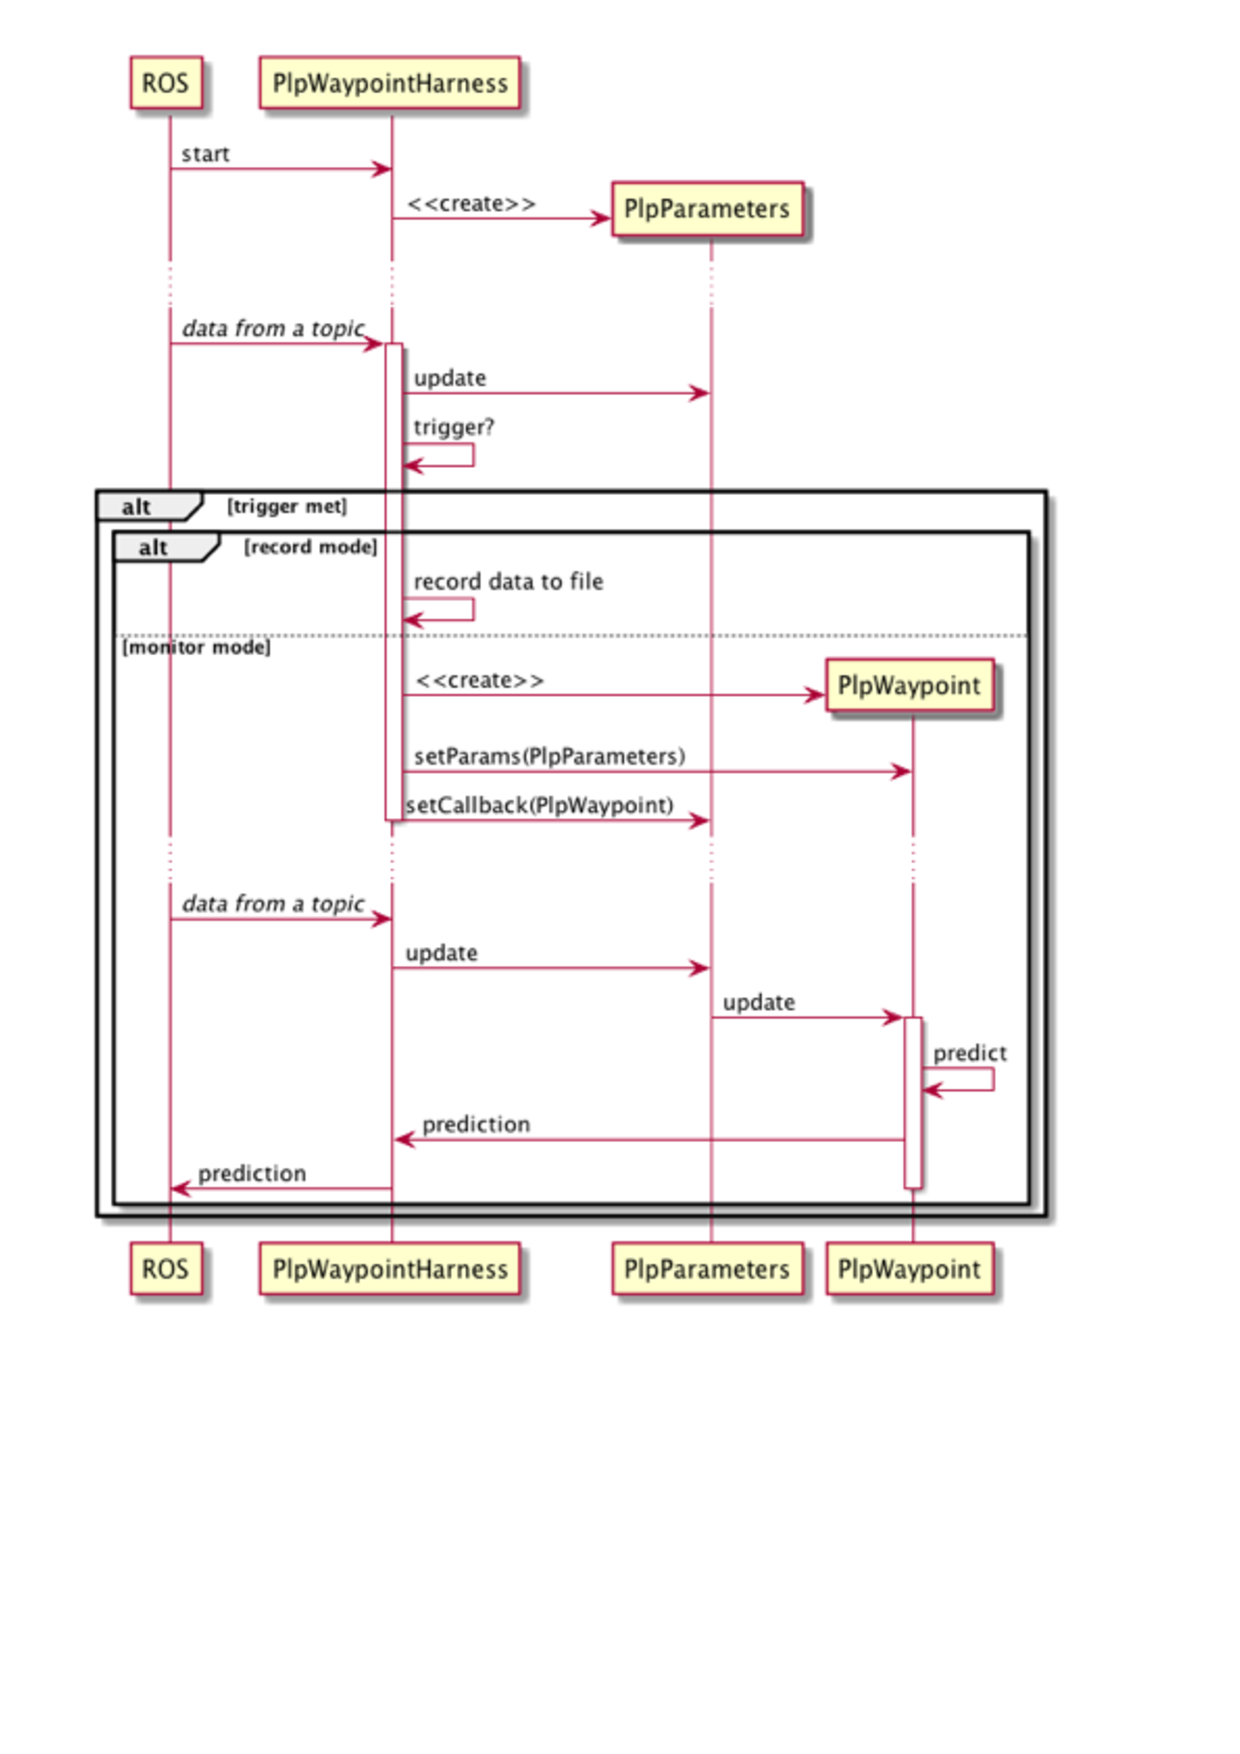
\includegraphics[scale=0.3]{code-generation}
%\vspace{-2.6cm}
%\caption{Event Diagram for PLP Generate Code}
%\label{fig:event-diagram}
%\vspace{-0.6cm}
%\end{figure}

\subsection{Code Generation for Data Gathering}
An important component of the PLP is a statistical profile of some of its properties, such as success rate and run-time distribution.
%and more ROS specific statistics, such as the rate in which messages are published or read.
 Our statistics collecting code is generated automatically from a PLP and is, in fact,
%works initially very much like the PLP code does. In fact, 
an operating mode of the aforementioned ROS harness node. When started in "data gathering mode", the ROS harness node records the parameters when the PLP's trigger condition becomes true. This allows for the following technique: run multiple simulations of a given task, with the ROS harness in data gathering mode. For each iteration, in addition to the file generated by the ROS harness node, record the final result (success, failure mode, run-time distribution, etc.). This
dataset can be used for predictive analysis using PLP parameters.

\subsection{Control Graph Verifier}

%\subsection{Play-outs and Planning}
%PLPs can be used for predicting the behavior of modules, and in particular, the behavior of module combinations, such as modules that run in sequence or in parallel, or in a loop. This calls for a theory of PLP composition, which is the subject of ongoing work. At present, we are focusing
%on predicting the success probability and run-time distribution of a set of PLP, run in sequence and in parallel
%Initial results on the complexity of exact and approximate computation of the success probability and run-time distribution for combinations
%of sequence and parallel execution of code associated with PLPs have been obtained (with exact computation being NP-hard, typically,
%and polytime approximation algorithms)~\cite{LiatMSC}
%For more complex settings, we use Monte-Carlo simulations. A tool for automatically computing these statistics is now implemented within the
%autonomous bob-cat project. At certain points, an operator may intervene, providing the bob-cat with a certain sequences of actions to perform.
%Using the PLPs of the component actions, our tool is able to predict the success probability and run-time distribution of the sequence.
%In difference to earlier work such as~\cite{Lesire11} which attempts to predict worst-case behavior, we are attempting to estimate distributions over running times, or their moments. 


\section{RELATED WORK}
PLPs for achievement goals are based on existing action languages. %, mixing features from a number of sources. 
Preconditions and effects go back to {\sc strips}~\cite{fikes:nilsson:ai-71}. 
Concurrency conditions, deterministic durations, and resources and their consumptions come with
PDDL2.1's temporal actions~\cite{PDDL2.1}. 
PLPs emphasize a slightly different version of concurrency condition, which attempts to address the issue of
action (here, module) interaction, introduced by~\cite{BB00}. Requiring exclusive use of a resource is 
a technique for preventing harmful interactions, or interactions whose effect cannot be predicted.
Thus, a module can require exclusive use of an arm, preventing other modules from interfering with its use,
an idea that goes back to classical mutexes in concurrent systems~\cite{Mutex}.
%, and is implemented in some languages for concurrent programming. 
A related idea appears in Structured Reactive Controllers~\cite{Beetz99} where the notion of embedability is defined. 
That notion asserts that a module may be executed concurrently with a set of other modules 
without their execution interfering with its ability to reach its goal. 

PLPs address uncertainty by borrowing ideas from
PPDDL~\cite{YouLit04} and RDDL~\cite{RDDL}. For each of these aspects (time, concurrency, uncertainty, resources) there are languages that provide more powerful constructs, whereas PLPs attempt to address all essential aspects of the performance of a module, while providing a good trade off between expressiveness and intuitiveness. Thus,
while PDDL2.1 can describe temporal actions, it cannot describe actions with stochastic durations, and while
RDDL describes probabilistic effects, it does not specify temporally extended actions, etc.

Maintenance goals are also a well known concept (e.g.,~\cite{PRS}). 
%In principle, a maintenance goal could be specified using a version of temporally extended actions~\cite{PDDL2.1} in which some effects of an action take place immediately at the beginning of its execution and are true
%throughout its execution. Such specification is a bit counter-intuitive, though, as maintain modules usually maintain a condition that is already true. %Thus, the action would have the condition to be maintained both as a precondition and an effect.  
{\em Detect\/} and {\em observe\/} modules, on the other hand, are motivated by the ideas of observation in POMDPs and contingent planning, whereas the ideas behind the {\em repeat\/} module, and in particular, the introduction of
input/output frequencies appear new, to the best of our knowledge.

%Overall, with the exception of {\em repeat\/}, none of the constructs underlying PLPs is new, but their combination covers essential aspects of robotics modules, and includes components essential to the proper operation and use of functional modules, while attempting to remains intuitive.

The formalism most similar to PLP in terms of its constructs is  PRS~\cite{PRS}. It has achieve, maintain, and observation goals, context conditions, and properties, which can mention resource consumption. But herein lies a fundamental difference.
PRS is part of a large set of languages for {\em building\/} robotic modules and controllers that have been developed and improved
over the years. Other well-known languages are TCA/TDL~\cite{TCA}, RPML~\cite{RPML},  BIP~\cite{BIP2}  %~\cite{BIP,BIP2} 
Genom~\cite{Genom}  or even synthesis based tools for automated controller generation, such as~\cite{KP10}.
%
%PLPs on the other hand are descriptive rather than prescriptive. This why they contain important information about expected 
%performance, such as success probability, expected running time, and expected progress that is missing from the above languages. 
%Such descriptions can be used as a more structured, machine readable, specification language, describing the performance that the designer seeks, or as the input to automated tools that utilize information about expected behaviour for monitoring, validation, or planning. However, 
%they are {\em not\/} a tool for programming robots.
%
%
PLPs are more modest in aims and are not a language or an architecture for building robots.
% -- they are not part of a complete robot architecture nor are they a language for building robots. 
Their aim is to enhance existing practices and existing code and allow added value services, such as monitoring code generation. 
They are descriptive rather than prescriptive, and for this reason, they contain important information about expected performance, such as success probability, expected running time, and expected progress -- missing from the above languages.  
%Such descriptions can be used as a more structured, machine readable, specification language, describing the performance that the designer seeks, or as the input to automated tools that utilize information about expected behaviour for monitoring, validation, or planning, but they are {\em not\/} a tool for programming robots. 
Much like Eiffel~\cite{Eiffel}, PLPs do not enforce their "contracts".
% although monitoring them, as we suggest, is supported.
%hat is, we rely on the fact that the PLP is a faithful specification of the written code, but we cannot guarantee it. 
Instead, we offer the ability to generate code that monitors the contract, and statistics gathering tools that can, to some extent, 
verify, or improve the correctness of this specification, but only probabilistically. 

Our automated monitoring code generation is conceptually similar to
%The importance of safety monitoring for autonomous robots to their future deployment is clear to the robotics community, and several  approaches for addressing this issue have been proposed. 
run-time verification~\cite{runtimeveri} which generates code from temporal logic properties.
These properties are not necessarily component centred, as in PLPs. Both are somewhat complementary to more complete, model-based
pre-design techniques for defining safety constraints and interventions, such as SMOF~\cite{SMOF} and~\cite{Woodman12}, while
%is a model-based method that requires, beyond safety constraints, some sort of a model of intervention actions and a transition system. It aims to identify warning states, which are still safe, but in which some intervention is required to prevent transitions into states the violate the constraint. PLP-generated
%monitors  are based on a limited specification of components, not an entire transition system. They are passive, in the sense that they only reports on abnormal behavior, and do not provide a mechanism for interventions, yet the monitors are can be generated automatically.
%\cite{Woodman12} offer a similar methodology for safety one that starts with a hazards analysis, definition of risk requirements and constraints, identifying how the 
%unsafe conditions can be avoided or reversed, and ending with a safety policy that intervenes when required. This approach is integrated into the entire design process, and is more powerful than PLP monitors. However, 
PLP-based monitoring makes post-design monitoring easy.


%The approach taken by PLPs is minimalist in the sense that it does not dictate (nor provide) particular architecture or tools for module construction. There is no doubt that tools such as BIP~\cite{BIP,BIP2} which provide a methodology for top-down construction of modules as well as tools for validating properties of the constructed system, or techniques for automated controller generation such as~\cite{KP10} provide more powerful support for the synthesis and construction of systems with guarantees. 
%Nevertheless, little code is generated today using formal specification methods,
%and we expect that this state of affairs will be true in the area of robot design. On the other hand, software engineering methods are commonly used in the design of large software systems. PLPs and the provide a specification method that is similar in some ways to the commonly used SSS, yet more formal, and fits well within a methodology in which a systems engineer provides an abstract, almost textual specification, that is then implemented in code by a programmer.  They also provide a way for a designer to explain/guarantee the functional behavior of its module at some level.
%
%
%Another line in plan representation is based on the concept of reacting to
%conditions in the real world, in the form of Structured Reactive Plans (SRPs)
%\cite{Beetz00}. SRPs build upon the notion of Firby's Reactive Action Packages
%(RAPs) \cite{Firby87}, in order to create a plan-like representation of a program,
%while allowing for opportunistic actions and numerous other real-time interactions.
%SRPs also have other derivatives and applications, such as Structured Reactive Controllers (SRCs)
%\cite{Beetz99}.
%
%Although we have not closely investigated the relationship between PLPs and SRPs, several
%differences are evident.
%The way the trigger conditions for plans are expressed in SRCs looks similar
%to the way preconditions are expressed in the PLAs presented in the current paper.
%However, the semantics are different as in SRCs the action is applied as soon as the
%conditions are met, whereas in PLAs this is not implied, the effects will occur only
%{\em if} the action will occur under the given condition. That is, these notions are
%orthogonal and one might envision defining PLAs on to of SRPs as well, although we have not
%looked into how this might be done. Additionally, PLPs are designed with explicit representation of
%uncertainty, which was not a goal in SRPs, but possibly that could also be added to SRP in
%a manner similar to the way PLPs extend classical planning languages.
%

\section{SUMMARY AND FUTURE WORK}
%\note{To be updated}
We described {\em performance level profiles\/},
a language for specifying the expected performance of functional modules. PLPs are motivated by the need to provide more precise, quantifiable,  machine-readable descriptions of module behavior. With such information, one can detect abnormal behavior, generate monitoring code automatically, and provide clear guarantees to users.
We developed a set of tools for building PLPs and using them for performance monitoring, and are currently working
on tools that automatically generate code from PLPs in support of automated planning~\cite{PlanRob16}.

%Our original motivation stems from discussions with our industry partners who lack a language and a methodology for providing their clients with reasonable performance guarantees for their products. This has led us to suggest the idea of {\em performance-level agreements} (PLA)
%a notion inspired by service-level agreements, common in telecommunications industry and in the area of web services. As robots, and especially autonomous robots operate in a much more open-ended environment, a much richer language is required for
%their formulation. 

PLPs attempt to make action description language more intuitive and appropriate for robotics applications,
using well known notions of achievement and maintenance goals, analogous notions for the sensing-side of robot activity, 
expected progress rates, and the {\em repeat\/} option which helps model the  notions of frequency and latency.
%commonly used by designers of robotic hardware and software.

% -- being able to provide operators with useful information about unexpected or problematic conditions, such as modules operating without the required preconditions and concurrent conditions, information about running times, and effects of modules used online. We are now working 
%In addition, we have worked on the idea of automated composition of PLPs, to provide the support needs for validation and, eventually planning.

In defining PLPs we preferred intuitiveness and expressiveness over economy and succinctness. We envision that future use will lead to additional fields describing properties that are useful to know.
%being included in PLPs and see this as a plus. For example, 
%we are now considering issues such as partial success capturing the idea of that some modules, in case they cannot achieve 
%their desired goal, e.g., because some condition is violated, will nevertheless attempt to achieve an alternative goal, or perhaps,
%to ensure a safe end-state.
Our point is that users can always decide not to specify certain aspects of their module, and automated reasoning tools can always use only a subset of the information. For example, for generating PDDL planning domains, we use only part of information in the PLP. If a stronger planner is available, a compiler to a more informative action description language can be used, instead.



%To realize these possible benefits, the PLP definition may require farther enhancement to cover
%additional aspects of module performance. 
%For example, we are now considering issues such as partial success -- e.g., sometimes a module that is unable
%to achieve its desired goal, e.g., because of some condition that is violated, 
%may still be able to achieve an alternative one, or perhaps ensure some safe end-state. 
%Similarly, often modules are designed with a back-up module that is called in the case of failure.
%While each such module can be specified independently, it may be desirable to have a special structure for module/backup pairs. Another possible enhancement is a more refined process model. Some modules, provide more complex services that require modeling some notion of state. Indeed, many of the formal tools developed for principled construction of robotic modules supply such a model, e.g., a state-machine~\cite{BIP2} or a Petri-Net~\cite{Montano00}.
%We wish PLPs to remain abstract specification and not nearly executable process models. Yet, the exact level of abstraction
%that will provide sufficient functionality remains an open question for future research.\\

%Finally, one important thread of current work is providing PLPs with a formal semantics by mapping them into temporal logic formulas. Ideas such as achieve, maintain, repeat, as well as frequencies, can be modeled using formulas in a suitable temporal logic. Similarly, preconditions, concurrency conditions, termination conditions etc., can also be modeled this way. Combining this information together and using a suitable theorem prover or model checker (such as PRISM~\cite{PRISM}, which support probabilistic temporal logic) can enable us to formally prove properties of a system using the PLPs of its components. Providing more added value to PLPs.\\



\addtolength{\textheight}{-12cm}   % This command serves to balance the column lengths
                                  % on the last page of the document manually. It shortens
                                  % the textheight of the last page by a suitable amount.
                                  % This command does not take effect until the next page
                                  % so it should come on the page before the last. Make
                                  % sure that you do not shorten the textheight too much.

%%%%%%%%%%%%%%%%%%%%%%%%%%%%%%%%%%%%%%%%%%%%%%%%%%%%%%%%%%%%%%%%%%%%%%%%%%%%%%%%



%%%%%%%%%%%%%%%%%%%%%%%%%%%%%%%%%%%%%%%%%%%%%%%%%%%%%%%%%%%%%%%%%%%%%%%%%%%%%%%%



%%%%%%%%%%%%%%%%%%%%%%%%%%%%%%%%%%%%%%%%%%%%%%%%%%%%%%%%%%%%%%%%%%%%%%%%%%%%%%%%
%\section*{APPENDIX}

%Appendixes should appear before the acknowledgment.

\section*{ACKNOWLEDGMENT}
We are grateful to our ROBIL  colleagues for their useful input and help. This work was supported by MAFAT's ROBIL project, ISF Grant 933/13, 
the Helmsley Charitable Trust through the Agricultural, Biological and Cognitive Robotics Center of Ben-Gurion University of the Negev, and the Lynn and William Frankel Center for Computer Science.

%%%%%%%%%%%%%%%%%%%%%%%%%%%%%%%%%%%%%%%%%%%%%%%%%%%%%%%%%%%%%%%%%%%%%%%%%%%%%%%%

\bibliographystyle{elsarticle-num-names}
%%\bibliographystyle{IEEEtran} 
\bibliography{all.bib}   

%\appendix{}
%\listoftodos{}

\end{document}
